\section{Capture et traitement du flux vidéo}
Une fois le pont réseau Sub-1 GHz établi, le défi consiste à formater la source vidéo pour qu'elle puisse
traverser ce canal étroit sans générer de goulots d'étranglement. Cette section détaille les choix
logiciels, l'optimisation des paramètres de compression, et la gestion des tampons matériels.

\subsection{Arbitrage entre les normes H.264 et H.265}
Le choix initial du projet s'était porté sur la norme \textbf{H.265 (HEVC)}. Successeur du H.264, elle 
offre une efficacité de compression supérieure de 50\%, permettant de maintenir une image nette même à 
des débits très faibles (400 kbps). Cependant, cette complexité algorithmique exige des ressources de 
décodage importantes.

Lors des phases de tests sur la station de réception finale (Raspberry Pi 4), l'absence d'un pilote de 
décodage matériel H.265 stable et performant sous Linux (\texttt{v4l2h265dec}) a provoqué une latence 
très élevée, dépassant les 300 ms. 

Le système a donc été \textit{downgradé} vers la norme \textbf{H.264 (AVC)}. Bien que moins performante 
en termes de ratio qualité/débit, elle bénéficie d'un support matériel universel. Ce choix a permis
d'exploiter un décodage extrêmement rapide sur Raspberry Pi, ramenant la latence de traitement au niveau 
de la milliseconde tout en conservant une fluidité d'image compatible avec le pilotage FPV.

\subsection{Le framework GStreamer et l'optimisation H.264}
Pour gérer le traitement, la compression et l'encapsulation de la vidéo, le framework \textit{open-source} 
GStreamer\index{GStreamer} a été retenu comme outil principal de l'architecture. Son approche modulaire 
permet de relier directement la sortie d'un composant matériel à un autre, en minimisant les copies en 
mémoire vive (\textit{Zero-Copy}).

Bien que l'acquisition sur Raspberry Pi ait nécessité le recours ponctuel à un outil natif, la logique de 
compression du flux exploite universellement la norme H.264. La stratégie de configuration globale a été 
pensée pour prioriser la vitesse d'exécution au détriment de la qualité visuelle.

\newpage

\subsection{Pipelines d'émission (TX)}
\begin{figure}[htbp]
    \centering
    
\includegraphics[width=1\textwidth]{imgs/complet_schematic_nb2.png}
    \caption{(2) Capture vidéo}
    \label{fig:complet_schematic_nb3}
\end{figure}
Pour implémenter cette stratégie de très basse latence en situation réelle, les chaînes de traitement 
ont été développées et adaptées selon l'architecture matérielle cible. 

Lors des premiers essais sur la Raspberry Pi 4B, il a été constaté que l'utilisation de l'encodeur 
matériel intégré au travers du plugin GStreamer standard (\texttt{v4l2h264enc}) introduisait une latence 
inacceptable. L'empilement logiciel et la gestion des mémoires tampons du pilote V4L2 ralentissaient 
fortement l'acquisition.

Pour la plateforme Raspberry Pi, GStreamer a donc été écarté à l'émission au profit de l'outil 
natif \texttt{rpicam-vid}. Basé sur \textit{libcamera}, il permet un accès direct et optimisé au 
processeur de traitement d'image (ISP) et à l'encodeur matériel (H.264) de la carte, réduisant 
drastiquement le temps de traitement.

\begin{lstlisting}[language=bash]
# Sur Nvidia Jetson Nano (NVENC)
gst-launch-1.0 nvarguscamerasrc ! \
'video/x-raw(memory:NVMM),width=640,height=480,framerate=60/1' ! \
nvv4l2h264enc bitrate=400000 control-rate=1 preset-level=1 \
insert-sps-pps=true idrinterval=1000 maxperf-enable=1 num-B-Frames=0 ! \
h264parse ! fdsink

# Sur Raspberry Pi 4B (V4L2)
gst-launch-1.0 v4l2src device=/dev/video0 ! \
'video/x-raw,width=640,height=480,framerate=60/1' ! \
v4l2h264enc extra-controls="controls,video_bitrate=400000,video_b_frames=0" ! \
h264parse ! fdsink

# Sur Raspberry Pi 4B (Outil natif libcamera rpicam-vid)
rpicam-vid -t 0 --width 640 --height 480 --framerate 60 --bitrate 400000 \
--profile baseline --inline --intra 60 --flush -o -
\end{lstlisting}

\subsubsection{Précisions sur les paramètres d'envoi}
Certains drapeaux (\textit{flags}) spécifiques ont été ajoutés pour forcer le comportement temps réel des chaînes et leurs débits :
\begin{itemize}
\item \textbf{Le contrôle de débit strict (CBR) :} Le débit est verrouillé à 400 kbps 
    (\texttt{bitrate=400000}) pour éviter tout pic de données soudain qui saturerait le bus SPI 
    et la mémoire du STM32.
    \item \textbf{L'absence d'images bidirectionnelles :} Sur GStreamer, \texttt{num-B-Frames=0} est 
    explicitement appelé. Sur Raspberry Pi, l'utilisation du profil \texttt{--profile baseline} garantit 
    que l'encodeur ne génère aucune trame "B" nécessitant d'attendre l'image future, supprimant ainsi un 
    délai algorithmique.
    \item \textbf{L'espacement des images clés (I-Frames) :} L'envoi d'images clés, très volumineuses, 
    doit être contrôlé. Sur la Jetson, \texttt{idrinterval=1000} les espace au maximum. Sur la Raspberry Pi, 
    \texttt{--intra 60} force une image clé par seconde (à 60 fps) pour permettre au récepteur de raccrocher 
    rapidement en cas de perte de signal RF.
    \item \textbf{L'injection des en-têtes de flux :} Les arguments \texttt{insert-sps-pps=true} (Jetson) 
    et \texttt{--inline} (RPi) forcent l'encodeur à écrire les informations de séquence (SPS/PPS) à chaque 
    image clé. Sans cela, un récepteur subissant une micro-coupure réseau serait incapable de reprendre 
    le décodage du flux en cours de route.
    \item \textbf{L'expulsion immédiate des tampons (Flush) :} L'argument \texttt{--flush} sur \texttt{rpicam-vid} 
    garantit que les données H.264 sont immédiatement poussées dans la sortie standard (le *pipe* relié 
    à notre programme C) dès qu'elles sont prêtes, sans attendre de remplir un tampon logiciel de l'OS. 
    Sur GStreamer, c'est le \texttt{h264parse disable-passthrough=true} qui force cet alignement immédiat.
\end{itemize}

\newpage

\subsection{Pipelines de réception et d'affichage (RX)}
\begin{figure}[htbp]
    \centering
    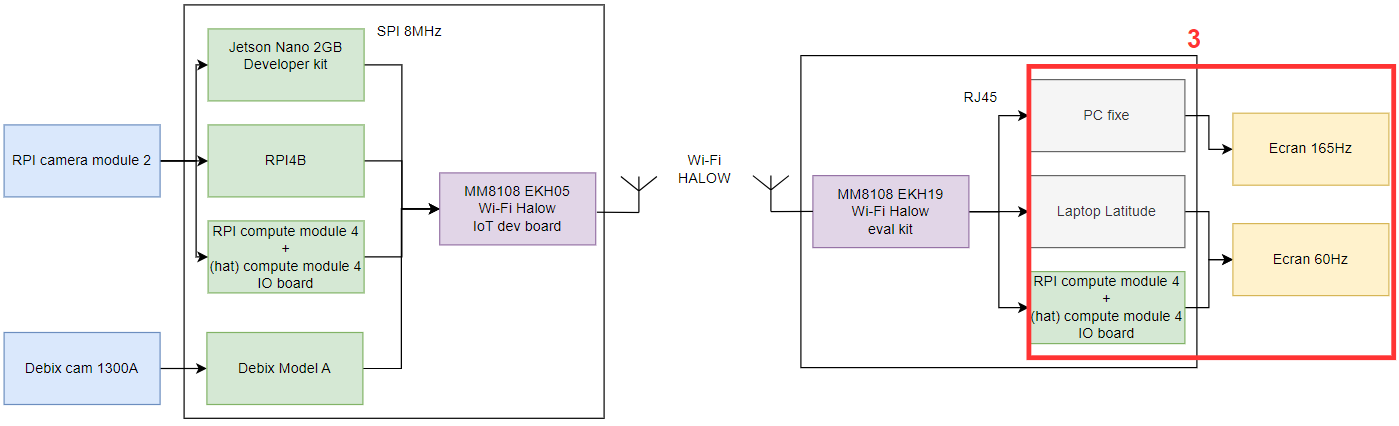
\includegraphics[width=1\textwidth]{imgs/complet_schematic_nb3.png}
    \caption{(3) Plateformes de traitement}
    \label{fig:complet_schematic_nb4}
\end{figure}
À la réception, le défi s'inverse : il faut décoder et afficher le plus vite possible. L'élément critique 
est \texttt{sync=false}, qui ordonne à GStreamer d'afficher chaque trame dès qu'elle est prête, en 
ignorant les horodatages.
\begin{lstlisting}[language=bash]
# Sur Station PC Windows (Acceleration D3D11)
gst-launch-1.0 udpsrc port=1337 buffer-size=0 ! \
"video/x-h264,width=640,height=480,stream-format=byte-stream" ! \
h264parse disable-passthrough=true ! d3d11h264dec ! \
queue max-size-buffers=1 leaky=downstream ! \
d3d11videosink sync=false async=false max-lateness=0

# Sur Station cible Raspberry Pi (Bare-Metal via KMS)
gst-launch-1.0 -v udpsrc address=0.0.0.0 port=1337 buffer-size=0 ! \
"video/x-h264,width=640,height=480,framerate=60/1,stream-format=byte-stream" ! \
h264parse disable-passthrough=true config-interval=-1 ! v4l2h264dec ! \
queue max-size-buffers=1 leaky=downstream ! \
kmssink sync=false max-lateness=0
\end{lstlisting}

\subsubsection{Précisions sur les paramètres de réception}
Tout comme pour la phase d'émission, l'arborescence des éléments logiciels de réception a été épurée de tout mécanisme de rétention ou de lissage temporel :
\begin{itemize}
    \item \textbf{\texttt{sync=false} :} Désactive la synchronisation sur l'horloge globale du pipeline. L'élément de rendu (\textit{sink}) affiche la trame 
    immédiatement dès sa réception au lieu de la retenir pour respecter l'horodatage (\textit{timestamps}) d'origine, supprimant ainsi tout délai d'attente artificiel.
    \item \textbf{\texttt{queue max-size-buffers=1 leaky=downstream} :} Limite la file d'attente à un unique paquet en mémoire. Si un retard d'affichage survient 
    et qu'une nouvelle trame se présente, l'ancienne est immédiatement écrasée et jetée en aval (\textit{leaky downstream}). Cela empêche l'accumulation de retard 
    (\textit{buffer bloat}) et force le flux à recoller instantanément au temps réel.
    \item \textbf{\texttt{async=false} :} Empêche le composant d'affichage de bloquer le pipeline en attendant une phase de pré-chargement (\textit{preroll}) lors du 
    changement d'état, garantissant un démarrage visuel instantané dès la détection des premiers paquets UDP.
    \item \textbf{\texttt{max-lateness=0} :} Indique au moteur de rendu de ne tolérer aucun retard de traitement. Associé à l'omission de la synchronisation, ce drapeau 
    force le pipeline à ignorer toute tentative de calcul de recalage temporel pouvant induire de la gigue.
\end{itemize}

\subsection{Outils de diagnostic réseau}
En complément de GStreamer, des utilitaires standards ont été employés pour le diagnostic du flux. 
\texttt{Netcat} (\texttt{nc}) a été utilisé pour rediriger manuellement les paquets UDP lors du 
prototypage, tandis que \texttt{tcpdump}\index{Tcpdump} a permis de capturer les trames à la volée 
sur les interfaces sans-fil pour valider la non-fragmentation des paquets HaLow.